\documentclass[11pt,a4paper]{article}

\usepackage[utf8]{inputenc}
\usepackage[T1]{fontenc}
\usepackage{mathpazo}
\usepackage[scaled=0.92]{helvet}
\usepackage[margin=1in]{geometry}
\usepackage{graphicx}
\usepackage{amsmath,amssymb,amsfonts}
\usepackage{booktabs}
\usepackage{tabularx}
\usepackage{setspace}
\usepackage{titlesec}
\usepackage{fancyhdr}
\usepackage{float}
\usepackage{caption}
\usepackage{microtype}
\usepackage{tikz}
\usepackage{xcolor}
\usepackage{listings}
\usepackage[hidelinks]{hyperref}

\usetikzlibrary{shapes.geometric, arrows.meta, positioning, calc, matrix, fit, backgrounds}

\setstretch{1.15}
\setlength{\parindent}{0pt}
\setlength{\parskip}{0.8em}
\sloppy

\titleformat{\section}{\normalfont\large\bfseries\sffamily}{\thesection}{1em}{}
\titleformat{\subsection}{\normalfont\normalsize\bfseries\sffamily}{\thesubsection}{1em}{}
\titleformat{\subsubsection}{\normalfont\normalsize\itshape\sffamily}{\thesubsubsection}{1em}{}

\pagestyle{fancy}
\fancyhf{}
\fancyhead[L]{\small\sffamily Vision dan Scope}
\fancyhead[R]{\small\sffamily\thepage}
\renewcommand{\headrulewidth}{0.4pt}

\captionsetup{font=small,labelfont=bf,labelsep=period}

\renewenvironment{abstract}
{\small
	\begin{center}\textbf{\sffamily Abstrak}\end{center}
	\begin{quote}}
	{\end{quote}}

\lstdefinestyle{code}{
	basicstyle=\ttfamily\small,
	frame=single,
	rulecolor=\color{black},
	breaklines=true,
	showstringspaces=false,
	columns=fullflexible,
	keepspaces=true,
	framesep=6pt,
	aboveskip=1em,
	belowskip=1em,
	xleftmargin=0pt
}

\lstdefinestyle{out}{
	basicstyle=\ttfamily\small,
	frame=tb,
	rulecolor=\color{black},
	breaklines=true,
	showstringspaces=false,
	columns=fullflexible,
	keepspaces=true,
	framesep=4pt,
	aboveskip=1em,
	belowskip=1em
}

\title{\vspace{-1.5cm}\textbf{\sffamily\LARGE Vision dan Scope\\ Kompas dan Rute Proyek Perangkat Lunak}}
\author{
	\textbf{Muhammad Riduwan Khafidi} \\
	\small Program Studi Teknik Rekayasa Perangkat Lunak \\
	\small Politeknik Negeri Batam \\
	\small \texttt{4342611034@students.polibatam.ac.id}
}
\date{\small\today}

\begin{document}

\maketitle
\thispagestyle{empty}

\begin{abstract}
	Makalah ini membahas dua konsep yang sering dicampur padahal berbeda secara fundamental: product vision dan product scope. Ia memberi tiga tes diagnosis untuk membedakan keduanya, menganalisis ulang kuis ``apakah ini perubahan vision'' dari slide kelas dengan lebih cermat, dan memperkenalkan ide bahwa scope creep bukan persoalan klien, melainkan persoalan disiplin analyst. Delapan visualisasi dan tiga tabel menyertai pembahasan, termasuk template Vision and Scope Document empat bagian serta lima proses Project Scope Management. Sebuah studi kasus sepuluh langkah dengan sistem reservasi lapangan futsal menunjukkan bagaimana vision dipecah menjadi scope per rilis, bagaimana WBS dipakai sebagai alat negosiasi, dan bagaimana setiap permintaan baru dijawab dengan tepat satu dari tiga kemungkinan: ya, tidak, atau rilis berikutnya.
\end{abstract}

\section{Pendahuluan}

\subsection{Analogi Pembuka}

Bayangkan seorang pendaki gunung. Ia membuka peta, menemukan puncak yang ingin ia tuju, dan menandainya dengan lingkaran merah. Puncak itu adalah \textbf{vision}. Ia tidak berubah meskipun ia salah jalan, kehabisan air, atau berpapasan dengan jalur alternatif.

Lalu ia menetapkan: hari ini saya akan mendaki dari basecamp ke shelter satu. Besok dari shelter satu ke shelter dua. Lusa dari shelter dua ke puncak. Rute-rute harian ini adalah \textbf{scope}. Mereka bisa berubah kapan saja, tergantung cuaca, kondisi fisik, atau informasi baru dari pendaki lain yang baru turun.

Pendaki yang tidak punya puncak akan berjalan berputar-putar. Pendaki yang tidak punya rute harian akan berjalan tanpa rencana dan kehabisan bekal di tengah jalan. Vision tanpa scope adalah mimpi. Scope tanpa vision adalah kesibukan tanpa arah.

\subsection{Mengapa Topik Ini Penting}

Slide kelas membuka dengan kalimat tajam: ``A project without a clearly defined vision and scope will be an unfocused and undirected project.'' Tapi kalimat itu belum menjelaskan \textit{mengapa} dua hal ini sering disalahpahami sebagai satu hal yang sama.

Di lapangan, banyak tim yang menyebut ``visi kami adalah membuat aplikasi kasir dengan fitur A, B, dan C''. Itu bukan vision. Itu scope yang sedang menyamar jadi vision. Ciri khasnya: begitu salah satu fitur dibatalkan, seluruh proyek terasa kehilangan arah. Tim yang benar-benar punya vision akan tetap tahu ke mana harus pergi meskipun satu fitur dibuang.

\subsection{Peta Pembahasan}

Makalah ini disusun berurutan. Bagian kedua membahas vision, termasuk tiga tes diagnosis. Bagian ketiga membahas scope dengan tiga tes yang setara. Bagian keempat menyatukan keduanya dalam model hierarki rilis. Bagian kelima memberi diagnosis untuk pola paling sering muncul: fitur yang masuk, keluar, lalu masuk lagi. Bagian keenam membahas cara mengukur scope. Bagian ketujuh membahas siapa yang berwenang menyelesaikan konflik requirement. Bagian kedelapan menyajikan template Vision and Scope Document. Bagian kesembilan membedah lima proses scope management. Bagian kesepuluh sampai kedua belas membahas ``is this in scope'', scope creep, dan kuis vision change dari slide. Bagian ketiga belas sampai kelima belas merangkum perbandingan, kesalahan umum, dan lembar rujukan cepat. Bagian keenam belas memandu studi kasus sepuluh langkah, dan bagian ketujuh belas menutup dengan tiga prinsip.

\section{Apa Itu Product Vision}

Product vision adalah arah jangka panjang produk. Fungsinya menyelaraskan seluruh stakeholder pada arah yang sama. Ia berlaku untuk produk secara keseluruhan, bukan untuk satu rilis tertentu. Biasanya ia tidak berubah untuk waktu yang lama.

Perhatikan Gambar~\ref{fig:compass}. Vision itu seperti kompas, bukan peta jalan.

\begin{figure}[H]
	\centering
	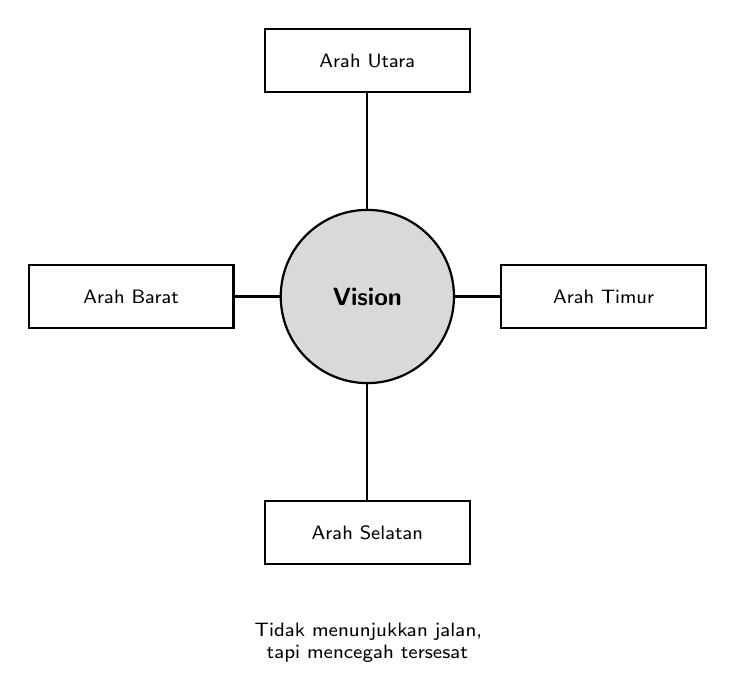
\begin{tikzpicture}[
			compbox/.style={circle, draw=black, thick, fill=black!15, minimum size=2.2cm, align=center, font=\sffamily\small\bfseries},
			direction/.style={rectangle, draw=black, thick, fill=white, minimum width=2.6cm, minimum height=0.8cm, align=center, font=\sffamily\scriptsize, inner sep=3pt},
			conn/.style={draw, thick}
		]
		\node[compbox] (c) at (0,0) {Vision};
		\node[direction] (n) at (0, 3)   {Arah Utara};
		\node[direction] (e) at (3, 0)   {Arah Timur};
		\node[direction] (s) at (0, -3)  {Arah Selatan};
		\node[direction] (w) at (-3, 0)  {Arah Barat};

		\draw[conn] (c) -- (n);
		\draw[conn] (c) -- (e);
		\draw[conn] (c) -- (s);
		\draw[conn] (c) -- (w);

		\node[font=\sffamily\scriptsize, text width=3cm, align=center] at (0, -4.4) {Tidak menunjukkan jalan,\\tapi mencegah tersesat};
	\end{tikzpicture}
	\caption{Vision sebagai kompas, bukan peta jalan.}
	\label{fig:compass}
\end{figure}

Kompas tidak memberi tahu Anda harus belok kiri di pertigaan mana. Ia memberi tahu Anda sedang menghadap ke mana. Begitu juga vision: ia tidak menentukan fitur apa yang dibangun minggu depan, tapi ia memberi tahu apakah fitur itu membawa Anda lebih dekat atau lebih jauh dari tujuan.

\subsection{Tiga Tes Diagnosis}

Bagaimana membedakan vision yang asli dari scope yang menyamar? Perhatikan Gambar~\ref{fig:three-tests}. Ada tiga pertanyaan yang bisa dipakai.

\begin{figure}[H]
	\centering
	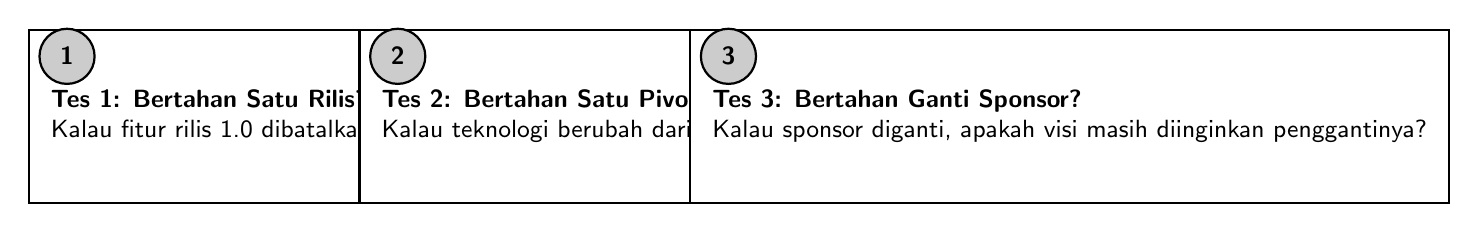
\begin{tikzpicture}[
			testbox/.style={rectangle, draw=black, thick, fill=white, minimum width=3.8cm, minimum height=2.2cm, align=left, font=\sffamily\small, inner sep=8pt},
			num/.style={circle, draw=black, thick, fill=black!20, minimum size=0.7cm, align=center, font=\sffamily\small\bfseries}
		]
		\node[testbox, anchor=north west] (t1) at (-6.3, 0) {
			\textbf{Tes 1: Bertahan Satu Rilis?} \\
			Kalau fitur rilis 1.0 dibatalkan semua, apakah visi masih berarti?
		};
		\node[testbox, anchor=north west] (t2) at (-2.1, 0) {
			\textbf{Tes 2: Bertahan Satu Pivot Teknologi?} \\
			Kalau teknologi berubah dari web ke mobile, apakah visi masih sama?
		};
		\node[testbox, anchor=north west] (t3) at (2.1, 0) {
			\textbf{Tes 3: Bertahan Ganti Sponsor?} \\
			Kalau sponsor diganti, apakah visi masih diinginkan penggantinya?
		};

		\node[num] at (-5.8, -0.35) {1};
		\node[num] at (-1.6, -0.35) {2};
		\node[num] at ( 2.6, -0.35) {3};
	\end{tikzpicture}
	\caption{Tiga tes untuk memastikan sesuatu itu vision asli, bukan scope yang menyamar.}
	\label{fig:three-tests}
\end{figure}

Kalau kalimat yang Anda tulis sebagai ``visi'' gagal lulus salah satu tes di atas, ia bukan vision. Ia scope yang ditulis terlalu jauh ke depan. Contoh visi yang gagal lulus Tes 1: ``Visi kami adalah membangun aplikasi kasir dengan modul inventori dan laporan penjualan.'' Buang modul inventori, dan visi itu sudah tidak berarti apa-apa. Visi yang lulus Tes 1 bisa jadi seperti ini: ``Visi kami adalah membuat pemilik toko kecil bisa mengelola keuangannya tanpa perlu belajar akuntansi.'' Ini tetap berarti meskipun modul inventori dihapus.

\subsection{Vision Conflict Diselesaikan oleh Siapa}

Business requirement yang dikumpulkan dari berbagai sumber bisa saling bertentangan. Contoh: pemilik toko ingin laporan yang detail, sementara kasir ingin tampilan yang sesederhana mungkin. Siapa yang memutuskan?

Jawaban di slide jelas: \textbf{project sponsor}, bukan developer. Developer yang memutuskan adalah developer yang akan disalahkan ketika hasilnya tidak sesuai harapan siapa pun. Sponsor adalah pihak yang paling tahu apa yang mereka butuhkan, karena merekalah yang menanggung konsekuensi bisnisnya.

Analyst dalam situasi ini bukan pengambil keputusan, tapi fasilitator. Ia memetakan konflik, menyajikan opsi, dan meminta sponsor memilih. Ini paralel dengan apa yang sudah dibahas di minggu ketiga: analyst memfasilitasi, bukan mengambil alih.

\section{Apa Itu Product Scope}

Product scope mengidentifikasi bagian dari proyek saat ini yang akan dikerjakan. Ia berlaku untuk iterasi spesifik yang akan diimplementasikan pada increment berikutnya. Scope lebih dinamis dari vision.

Kalau vision adalah kompas, scope adalah rute hari ini. Ia punya titik awal yang jelas (sumber daya saat ini), titik akhir yang jelas (apa yang akan dirilis), dan batas waktu yang jelas (kapan rilis itu terjadi).

Perhatikan Gambar~\ref{fig:window}. Scope itu seperti jendela, bukan dinding.

\begin{figure}[H]
	\centering
	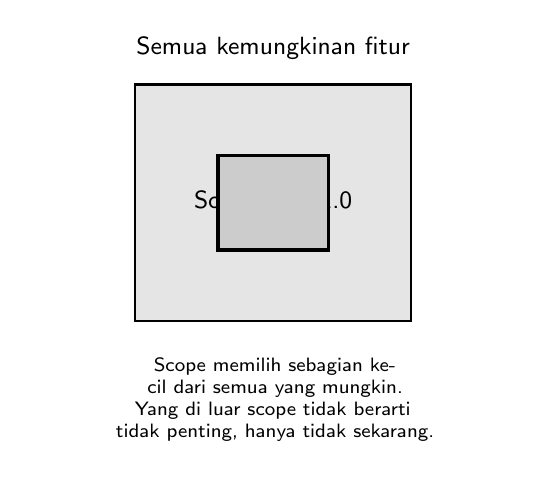
\begin{tikzpicture}[
			inbox/.style={rectangle, draw=black, thick, fill=black!10, minimum width=3.5cm, minimum height=3cm, align=center, font=\sffamily\small},
			outbox/.style={rectangle, draw=black, thick, dashed, fill=white, minimum width=3.5cm, minimum height=3cm, align=center, font=\sffamily\small},
			frame/.style={rectangle, draw=black, very thick, fill=black!20, minimum width=1.4cm, minimum height=1.2cm, align=center, font=\sffamily\bfseries}
		]
		\node[outbox] (all) at (0, 0) {};
		\node[font=\sffamily\small, anchor=south] at (0, 1.7) {Semua kemungkinan fitur};
		\node[inbox] (win) at (0, 0) {Scope Rilis 1.0};
		\node[frame] (ring) at (0, 0) {};

		\node[font=\sffamily\scriptsize, text width=6cm, align=center] at (0, -2.5) {Scope memilih sebagian kecil dari semua yang mungkin.\\Yang di luar scope tidak berarti tidak penting, hanya tidak sekarang.};
	\end{tikzpicture}
	\caption{Scope sebagai jendela yang memilih sebagian dari semua kemungkinan.}
	\label{fig:window}
\end{figure}

Yang di luar scope tidak sama dengan yang tidak penting. Ia hanya tidak dikerjakan pada iterasi saat ini. Perbedaan ini kecil tapi menentukan: kalau Anda mencampur keduanya, Anda akan menolak fitur bagus karena mengira fitur itu tidak penting, padahal hanya belum waktunya.

\subsection{Tiga Tes Diagnosis untuk Scope}

Sebagaimana vision punya tiga tes, scope juga punya tiga tes yang setara. Perhatikan Gambar~\ref{fig:scope-tests}.

\begin{figure}[H]
	\centering
	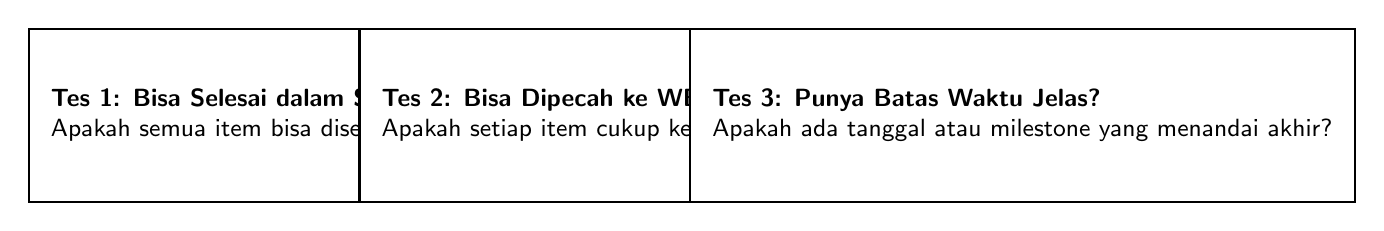
\begin{tikzpicture}[
			testbox/.style={rectangle, draw=black, thick, fill=white, minimum width=3.8cm, minimum height=2.2cm, align=left, font=\sffamily\small, inner sep=8pt}
		]
		\node[testbox, anchor=north west] (t1) at (-6.3, 0) {
			\textbf{Tes 1: Bisa Selesai dalam Satu Rilis?} \\
			Apakah semua item bisa diselesaikan dengan sumber daya dan waktu yang ada?
		};
		\node[testbox, anchor=north west] (t2) at (-2.1, 0) {
			\textbf{Tes 2: Bisa Dipecah ke WBS?} \\
			Apakah setiap item cukup kecil untuk jadi work package?
		};
		\node[testbox, anchor=north west] (t3) at (2.1, 0) {
			\textbf{Tes 3: Punya Batas Waktu Jelas?} \\
			Apakah ada tanggal atau milestone yang menandai akhir?
		};
	\end{tikzpicture}
	\caption{Tiga tes untuk memastikan scope-nya realistis dan terukur.}
	\label{fig:scope-tests}
\end{figure}

Kalau sesuatu gagal lulus Tes 1, ia bukan scope rilis ini, melainkan scope beberapa rilis ke depan. Kalau gagal lulus Tes 2, ia terlalu besar dan perlu dipecah. Kalau gagal lulus Tes 3, ia belum scope, masih harapan.

\section{Hierarki Vision dan Scope Rilis}

Satu product vision melingkupi banyak product scope. Setiap rilis punya scope-nya sendiri. Perhatikan Gambar~\ref{fig:hierarchy-release}.

\begin{figure}[H]
	\centering
	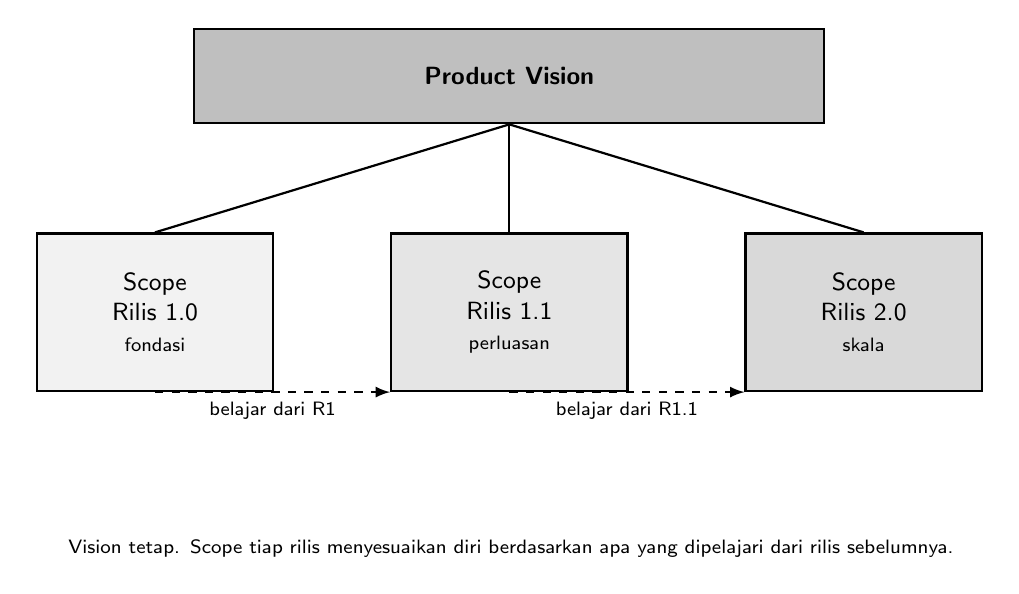
\begin{tikzpicture}[
			vbox/.style={rectangle, draw=black, thick, fill=black!25, minimum width=8cm, minimum height=1.2cm, align=center, font=\sffamily\small\bfseries},
			rbox/.style={rectangle, draw=black, thick, fill=black!10, minimum width=3cm, minimum height=2cm, align=center, font=\sffamily\small, inner sep=4pt},
			note/.style={font=\sffamily\scriptsize, text width=3cm, align=center},
			conn/.style={draw, thick}
		]
		\node[vbox] (v) at (0, 4) {Product Vision};

		\node[rbox, fill=black!5]  (r1) at (-4.5, 1)  {Scope\\Rilis 1.0\\{\scriptsize fondasi}};
		\node[rbox, fill=black!10] (r2) at (0, 1)     {Scope\\Rilis 1.1\\{\scriptsize perluasan}};
		\node[rbox, fill=black!15] (r3) at (4.5, 1)   {Scope\\Rilis 2.0\\{\scriptsize skala}};

		\draw[conn] (v.south) -- (r1.north);
		\draw[conn] (v.south) -- (r2.north);
		\draw[conn] (v.south) -- (r3.north);

		\draw[thick, -latex, dashed] (r1.south) -- (r2.south west) node[midway, below, font=\scriptsize\sffamily] {belajar dari R1};
		\draw[thick, -latex, dashed] (r2.south) -- (r3.south west) node[midway, below, font=\scriptsize\sffamily] {belajar dari R1.1};

		\node[font=\sffamily\scriptsize, text width=12cm, align=center] at (0, -2) {Vision tetap. Scope tiap rilis menyesuaikan diri berdasarkan apa yang dipelajari dari rilis sebelumnya.};
	\end{tikzpicture}
	\caption{Product vision melingkupi scope setiap rilis. Scope rilis berikutnya disesuaikan berdasarkan pembelajaran dari rilis sebelumnya.}
	\label{fig:hierarchy-release}
\end{figure}

Ada satu konsekuensi penting dari model ini yang sering terlewat: \textbf{scope rilis berikut tidak ditentukan di awal}. Ia ditentukan setelah rilis sebelumnya berjalan, ketika tim sudah punya data nyata tentang apa yang dipakai dan apa yang tidak. Ini yang disebut \textit{release treadmill}: setiap rilis memberi umpan balik yang mengubah scope rilis berikutnya, tapi tidak mengubah vision.

Tim yang menetapkan scope untuk semua rilis di awal adalah tim yang akan memaksa scope rilis 2.0 tetap sama meskipun data dari rilis 1.0 menunjukkan asumsi awalnya salah. Itu bukan disiplin, itu kekakuan.

\section{Tanda Vision Belum Cukup}

Slide kelas menyebut satu tanda yang sangat tajam: \textbf{business requirement belum cukup terdefinisi jika ada fitur yang awalnya dimasukkan, lalu dihapus, lalu dimasukkan lagi}. Perhatikan Gambar~\ref{fig:oscillation}.

\begin{figure}[H]
	\centering
	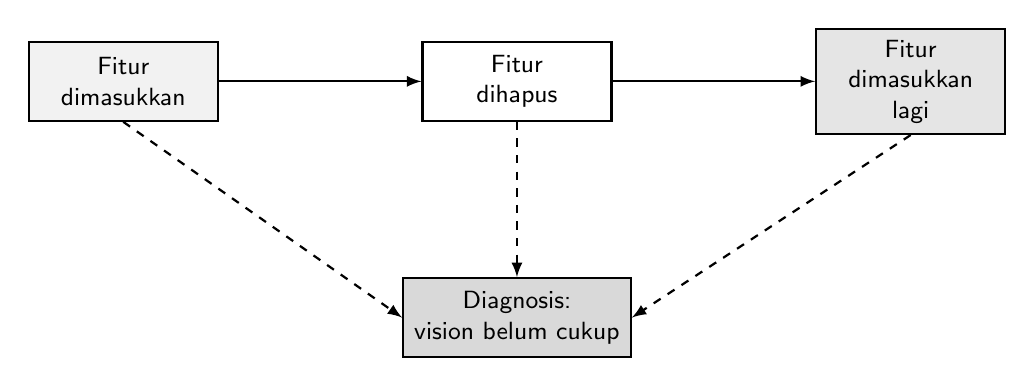
\begin{tikzpicture}[
			state/.style={rectangle, draw=black, thick, fill=white, minimum width=2.4cm, minimum height=1cm, align=center, font=\sffamily\small, inner sep=4pt},
			conn/.style={draw, thick, -latex},
			back/.style={draw, thick, -latex, dashed}
		]
		\node[state, fill=black!5]  (s1) at (0, 0)    {Fitur\\dimasukkan};
		\node[state, fill=white]    (s2) at (5, 0)    {Fitur\\dihapus};
		\node[state, fill=black!10] (s3) at (10, 0)   {Fitur\\dimasukkan\\lagi};
		\node[state, fill=black!15] (s4) at (5, -3)   {Diagnosis:\\vision belum cukup};

		\draw[conn] (s1) -- (s2);
		\draw[conn] (s2) -- (s3);
		\draw[back] (s3.south) -- (s4.east);
		\draw[back] (s1.south) -- (s4.west);
		\draw[back] (s2.south) -- (s4.north);
	\end{tikzpicture}
	\caption{Pola osilasi fitur yang menandakan vision belum cukup dalam.}
	\label{fig:oscillation}
\end{figure}

Analisis yang lebih dalam: osilasi ini bukan tanda scope yang salah. Ia tanda vision yang belum cukup dalam untuk memutuskan apakah fitur itu bagian dari arah atau bukan. Tanpa vision yang jelas, setiap fitur diuji dengan selera hari itu. Hari Senin terasa penting, hari Rabu terasa tidak, hari Jumat terasa penting lagi. Yang berubah bukan fiturnya, tapi selera yang menguji.

Solusinya bukan menulis scope lebih detail. Solusinya memperdalam vision sampai ia bisa menjawab satu pertanyaan sederhana untuk setiap fitur: fitur ini membawa kita lebih dekat ke arah yang kita tuju, atau tidak. Kalau vision cukup dalam, jawaban itu keluar dalam hitungan menit, bukan minggu.

\section{Mengukur Scope}

Slide menyebut empat cara mengukur scope. Perhatikan Gambar~\ref{fig:measure}.

\begin{figure}[H]
	\centering
	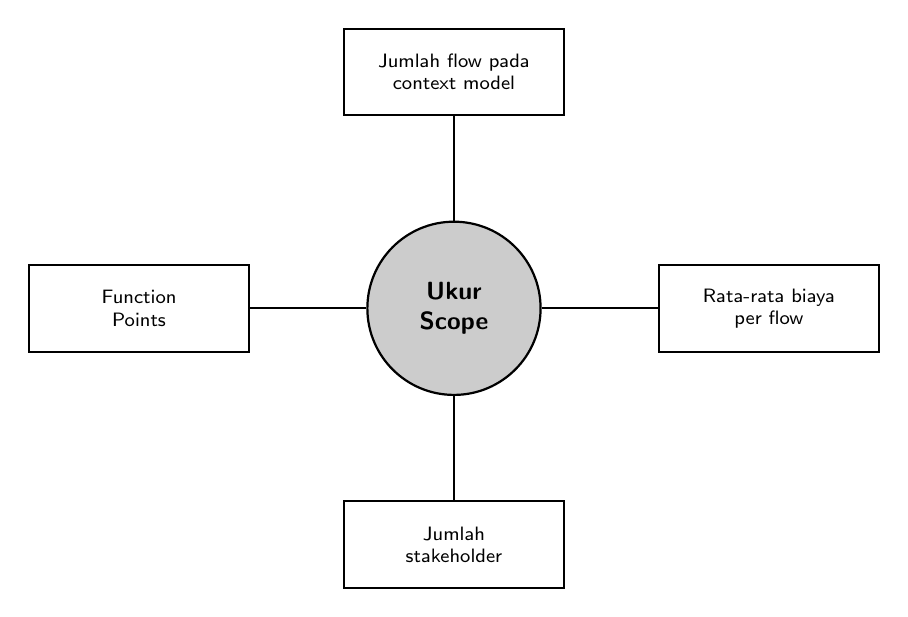
\begin{tikzpicture}[
			hub/.style={circle, draw=black, thick, fill=black!20, minimum size=2.2cm, align=center, font=\sffamily\small\bfseries},
			method/.style={rectangle, draw=black, thick, fill=white, minimum width=2.8cm, minimum height=1.1cm, align=center, font=\sffamily\scriptsize, inner sep=4pt},
			conn/.style={draw, thick}
		]
		\node[hub] (c) at (0,0) {Ukur\\Scope};

		\node[method] (m1) at (0,    3)   {Jumlah flow pada\\context model};
		\node[method] (m2) at (4,    0)   {Rata-rata biaya\\per flow};
		\node[method] (m3) at (0,   -3)   {Jumlah\\stakeholder};
		\node[method] (m4) at (-4,   0)   {Function\\Points};

		\draw[conn] (c) -- (m1);
		\draw[conn] (c) -- (m2);
		\draw[conn] (c) -- (m3);
		\draw[conn] (c) -- (m4);
	\end{tikzpicture}
	\caption{Empat cara mengukur scope.}
	\label{fig:measure}
\end{figure}

\textbf{Pertama, jumlah flow pada context model.} Context model adalah diagram yang menampilkan sistem sebagai satu kotak pusat, dengan panah masuk (input) dan panah keluar (output). Setiap panah adalah satu flow. Semakin banyak flow, semakin besar scope.

\textbf{Kedua, rata-rata biaya per flow.} Kalau satu flow rata-rata memakan 3 hari kerja, dan ada 20 flow, maka scope adalah sekitar 60 hari kerja. Ini estimasi kasar, tapi berguna untuk menolak scope yang tidak realistis di tahap awal.

\textbf{Ketiga, jumlah stakeholder.} Semakin banyak stakeholder, semakin banyak sudut pandang yang harus dipuaskan, semakin besar scope-nya.

\textbf{Keempat, Function Points.} Metode pengukuran yang menghitung jumlah input, output, query, file internal, dan file eksternal dari suatu sistem. Metode ini lebih formal dan sering dipakai di proyek enterprise.

Keempat cara ini tidak harus dipakai semua. Pilih satu atau dua yang paling cocok dengan konteks proyek, dan gunakan secara konsisten.

\section{Template Vision and Scope Document}

Vision and Scope Document mengumpulkan business requirement ke dalam satu dokumen yang menjadi fondasi pengembangan produk. Pemilik dokumen ini biasanya project sponsor. Project sponsor bekerja bersama development team atau analyst untuk membuatnya.

Dokumen ini punya empat bagian dengan empat belas subbagian. Perhatikan Tabel~\ref{tab:template}.

\begin{table}[H]
	\centering
	\caption{Template Vision and Scope Document empat bagian.}
	\label{tab:template}
	\footnotesize
	\begin{tabularx}{\textwidth}{l X}
		\toprule
		Bagian                    & Subbagian dan Isi                                                                                                                        \\
		\midrule
		1. Business Requirements  & 1.1 Background, 1.2 Business Opportunity, 1.3 Business Objectives and Success Criteria, 1.4 Customer or Market Needs, 1.5 Business Risks \\
		2. Vision of the Solution & 2.1 Vision Statement, 2.2 Major Features, 2.3 Assumptions and Dependencies                                                               \\
		3. Scope and Limitations  & 3.1 Scope of Initial Release, 3.2 Scope of Subsequent Releases, 3.3 Limitations and Exclusions                                           \\
		4. Business Context       & 4.1 Stakeholder Profiles, 4.2 Project Priorities, 4.3 Operating Environment                                                              \\
		\bottomrule
	\end{tabularx}
\end{table}

Bagian 1 dan 2 menjelaskan \textbf{mengapa dan apa}. Bagian 3 dan 4 menjelaskan \textbf{seberapa banyak dan dengan siapa}. Dokumen ini bukan technical specification. Ia tidak menjelaskan bagaimana sistem dibangun. Ia hanya menjelaskan apa yang akan dicapai, untuk siapa, dalam batas apa.

\section{Lima Proses Project Scope Management}

Project scope management punya lima proses yang membentuk satu siklus. Perhatikan Gambar~\ref{fig:five-processes}.

\begin{figure}[H]
	\centering
	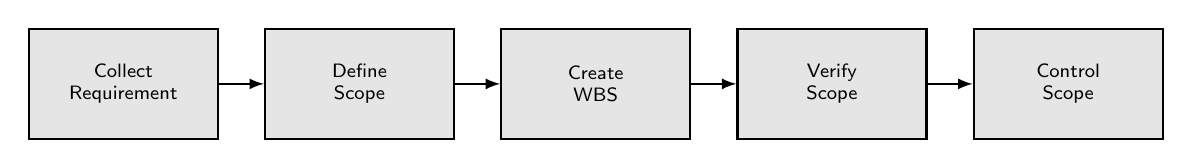
\begin{tikzpicture}[
			procbox/.style={rectangle, draw=black, thick, fill=black!10, minimum width=2.4cm, minimum height=1.4cm, align=center, font=\sffamily\scriptsize, inner sep=3pt},
			conn/.style={draw, thick, -latex}
		]
		\node[procbox] (p1) at (0, 0)    {Collect\\Requirement};
		\node[procbox] (p2) at (3, 0)    {Define\\Scope};
		\node[procbox] (p3) at (6, 0)    {Create\\WBS};
		\node[procbox] (p4) at (9, 0)    {Verify\\Scope};
		\node[procbox] (p5) at (12, 0)   {Control\\Scope};

		\draw[conn] (p1) -- (p2);
		\draw[conn] (p2) -- (p3);
		\draw[conn] (p3) -- (p4);
		\draw[conn] (p4) -- (p5);
	\end{tikzpicture}
	\caption{Lima proses project scope management.}
	\label{fig:five-processes}
\end{figure}

\textbf{Collect Requirement.} Mendefinisikan dan mendokumentasikan kebutuhan stakeholder untuk memenuhi tujuan proyek.

\textbf{Define Scope.} Mengembangkan deskripsi detail dari proyek dan produk. Hasilnya adalah scope statement yang jelas.

\textbf{Create WBS.} Memecah deliverable dan pekerjaan proyek menjadi komponen yang lebih kecil dan bisa dikelola. WBS adalah singkatan dari Work Breakdown Structure.

\textbf{Verify Scope.} Memformalkan penerimaan deliverable yang sudah selesai. Ini bukan uji coba teknis, tapi persetujuan formal dari pihak yang berwenang.

\textbf{Control Scope.} Memantau status dan mengelola perubahan pada baseline scope, baik untuk produk maupun proyek.

Yang sering terlewat adalah \textbf{Create WBS}. Banyak tim menganggap WBS sebagai dokumen teknis yang hanya dibutuhkan project manager. Padahal WBS adalah alat negosiasi paling ampuh dalam scope management. Ketika sponsor meminta tambahan fitur, analyst bisa membuka WBS dan berkata: ``Ini yang sudah ada di dalam 3 bulan. Kalau fitur ini ditambahkan, salah satu dari tiga item ini harus dikeluarkan, atau timeline bertambah.''

WBS memaksa percakapan tentang trade-off menjadi konkret. Tanpa WBS, percakapan selalu berakhir dengan ``kita coba dulu'' — yang artinya ``kita akan menyelesaikannya dengan lembur, meskipun tidak akan selesai tepat waktu.''

\section{Keeping Scope in Focus}

Setiap kali ada permintaan requirement baru, analyst wajib bertanya satu pertanyaan: \textbf{``Is this in scope?''} Perhatikan Gambar~\ref{fig:in-scope}.

\begin{figure}[H]
	\centering
	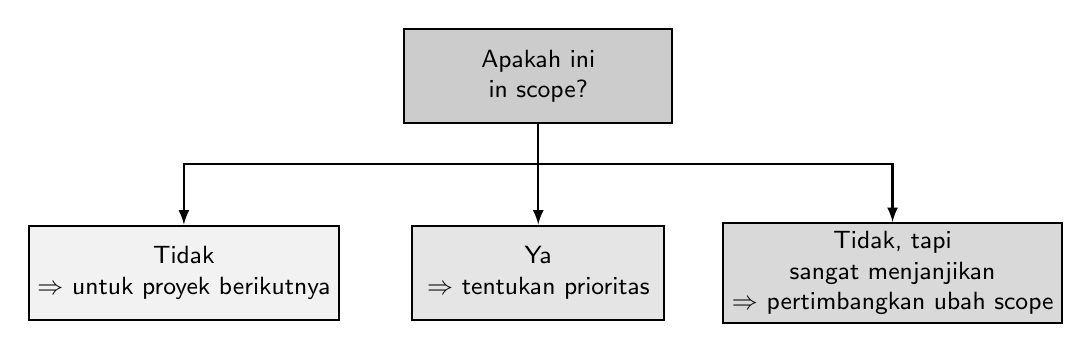
\begin{tikzpicture}[
			qnode/.style={rectangle, draw=black, thick, fill=black!20, minimum width=3.4cm, minimum height=1.2cm, align=center, font=\sffamily\small, inner sep=4pt},
			anode/.style={rectangle, draw=black, thick, fill=white, minimum width=3.2cm, minimum height=1.2cm, align=center, font=\sffamily\small, inner sep=3pt},
			conn/.style={draw, thick, -latex},
			lbl/.style={font=\sffamily\scriptsize}
		]
		\node[qnode] (q) at (0, 4) {Apakah ini\\in scope?};

		\node[anode, fill=black!5]  (no)   at (-4.5, 1.5)  {Tidak\\$\Rightarrow$ untuk proyek berikutnya};
		\node[anode, fill=black!10] (yes)  at (0, 1.5)     {Ya\\$\Rightarrow$ tentukan prioritas};
		\node[anode, fill=black!15] (next) at (4.5, 1.5)   {Tidak, tapi\\sangat menjanjikan\\$\Rightarrow$ pertimbangkan ubah scope};

		\draw[conn] (q.south) -- ++(0, -0.5) -| (no.north);
		\draw[conn] (q.south) -- (yes.north);
		\draw[conn] (q.south) -- ++(0, -0.5) -| (next.north);
	\end{tikzpicture}
	\caption{Tiga kemungkinan jawaban atas pertanyaan ``is this in scope?''.}
	\label{fig:in-scope}
\end{figure}

\textbf{Jika di luar scope tapi menarik}: catat untuk proyek berikutnya. Jangan buang, jangan kerjakan sekarang.

\textbf{Jika di dalam scope}: tentukan prioritasnya dibanding requirement lain. Bisa jadi ia masuk rilis ini, bisa jadi ia menggeser requirement lain yang lebih rendah prioritas.

\textbf{Jika di luar scope tapi sangat menjanjikan}: pertimbangkan untuk mengubah scope proyek. Ini keputusan berat, dan hanya sponsor yang bisa mengambilnya. Analyst memfasilitasi.

Perhatikan bahwa ada tiga jawaban, bukan dua. Sebagian besar analyst pemula hanya punya dua jawaban: ya atau tidak. Padahal jawaban ketiga — ``sangat menjanjikan tapi tidak untuk sekarang'' — adalah jawaban yang menyelamatkan hubungan dengan sponsor. Ia menunjukkan bahwa Anda serius mendengarkan, tapi juga serius menjaga scope.

\section{Scope Creep dan Cara Menanganinya}

Scope creep adalah pertumbuhan scope yang tidak terkendali. Ia terjadi ketika permintaan baru diterima tanpa perubahan timeline, anggaran, atau kualitas yang sepadan. Perhatikan Gambar~\ref{fig:creep}.

\begin{figure}[H]
	\centering
	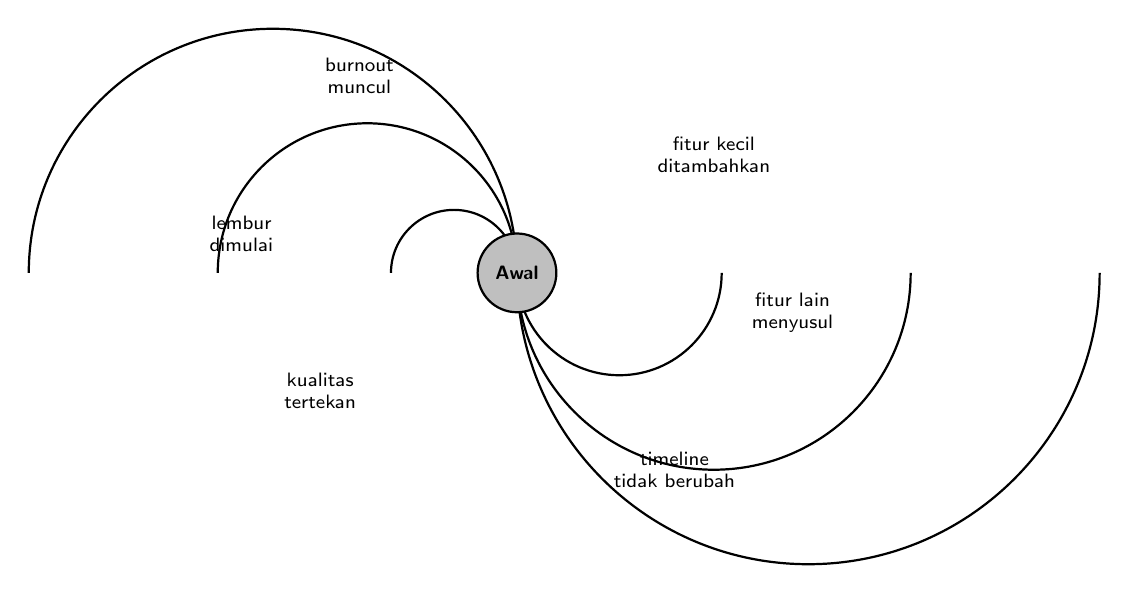
\begin{tikzpicture}[
			pivot/.style={circle, draw=black, thick, fill=black!25, minimum size=1cm, align=center, font=\sffamily\scriptsize\bfseries},
			spiral/.style={draw, thick},
			note/.style={font=\sffamily\scriptsize, text width=2.6cm, align=center}
		]
		\draw[spiral] (0,0) arc (0:180:0.8);
		\draw[spiral] (0,0) arc (180:360:1.3);
		\draw[spiral] (0,0) arc (0:180:1.9);
		\draw[spiral] (0,0) arc (180:360:2.5);
		\draw[spiral] (0,0) arc (0:180:3.1);
		\draw[spiral] (0,0) arc (180:360:3.7);

		\node[pivot] (c) at (0,0) {Awal};

		\node[note] at (2.5, 1.5) {fitur kecil\\ditambahkan};
		\node[note] at (3.5, -0.5) {fitur lain\\menyusul};
		\node[note] at (2.0, -2.5) {timeline\\tidak berubah};
		\node[note] at (-2.5, -1.5) {kualitas\\tertekan};
		\node[note] at (-3.5, 0.5) {lembur\\dimulai};
		\node[note] at (-2.0, 2.5) {burnout\\muncul};
	\end{tikzpicture}
	\caption{Spiral scope creep yang mulai dari fitur kecil dan berakhir pada kelelahan tim.}
	\label{fig:creep}
\end{figure}

Slide menyebut enam respons terhadap scope creep:
\begin{enumerate}
	\item Minta klien memprioritaskan requirement.
	\item Buat ekspektasi jelas.
	\item Gambarkan scope bersama klien.
	\item Selalu tanya ``is this in scope?''.
	\item Perpanjang jadwal proyek.
	\item Tambah biaya proyek.
\end{enumerate}

Tapi ini belum menjawab akar masalahnya. Akar scope creep bukan klien yang terus meminta. Akar scope creep adalah analyst yang tidak punya sistem untuk menolak dengan elegan. Kalau setiap permintaan baru dijawab dengan ``kita coba dulu'', maka setiap permintaan pada akhirnya akan dikerjakan, dan spiral pada Gambar~\ref{fig:creep} dimulai.

Analyst yang punya sistem menjawab setiap permintaan dengan tepat satu dari tiga kata: \textbf{ya}, \textbf{tidak}, \textbf{rilis berikutnya}. Tidak ada kata keempat seperti ``mungkin'' atau ``kita lihat nanti''. Kata-kata itu adalah cara paling halus untuk memulai scope creep.

Perhatikan pula satu jebakan yang sering muncul: \textit{sunk cost fallacy}. Tim kadang menolak membuang fitur yang sudah setengah jadi meskipun fitur itu di luar scope. Alasan yang muncul: ``sudah terlanjur dikerjakan, sayang kalau dibuang.'' Padahal kode yang tidak dipakai adalah technical debt yang terus menua. Membuangnya sekarang lebih murah daripada memeliharanya selama tiga tahun.

\section{Analisis Kuis Vision Change}

Slide memberi kuis dengan empat pilihan. Perhatikan Tabel~\ref{tab:vision-quiz}.

\begin{table}[H]
	\centering
	\caption{Analisis kuis vision change dari slide kelas.}
	\label{tab:vision-quiz}
	\footnotesize
	\begin{tabularx}{\textwidth}{l X X}
		\toprule
		Pilihan                                                                                & Analisis                                                                                                                                & Kesimpulan                 \\
		\midrule
		A. Klien pindah dari mobile gaming ke virtual reality                                  & Tergantung bagaimana vision ditulis. Kalau visi ``game imersif'', VR adalah scope. Kalau visi ``game mobile'', VR adalah vision change. & Ambigu, tergantung rumusan \\
		B. Tim mengubah detail implementasi produk                                             & Detail implementasi adalah ranah scope, bukan vision.                                                                                   & Bukan vision change        \\
		C. Proyek kelebihan anggaran, dipaksa dihentikan sementara                             & Ini masalah constraint, bukan vision.                                                                                                   & Bukan vision change        \\
		D. Klien mengubah produk dari game project management menjadi aplikasi desain furnitur & Domain produk berubah total. Visi lama tidak lagi relevan.                                                                              & Vision change              \\
		\bottomrule
	\end{tabularx}
\end{table}

Kunci jawaban yang biasa diberikan adalah \textbf{A dan D}. Tapi analisis di Tabel~\ref{tab:vision-quiz} menunjukkan sesuatu yang lebih menarik: pilihan A sebenarnya ambigu. Ia hanya menjadi vision change jika vision statement-nya secara eksplisit menyebut ``mobile''. Kalau vision statement-nya menyebut ``game imersif untuk profesional muda'', maka VR adalah salah satu rute, bukan perubahan tujuan.

Pelajaran dari analisis ini: \textbf{jawaban atas pertanyaan ``apakah ini vision change'' bergantung pada bagaimana vision ditulis}. Ini bukan kelemahan kuis, ini kekuatan kuis. Ia menunjukkan bahwa vision statement yang ditulis dengan buruk akan menghasilkan kebingungan bahkan pada pertanyaan sesederhana ini.

Pilihan D tidak ambigu. Nama domain berubah dari game ke furnitur. Tidak ada rumusan vision yang bisa menutupi fakta bahwa dua hal ini adalah dua produk yang berbeda.

\section{Perbandingan Ringkasan}

Tabel~\ref{tab:summary} merangkum perbedaan kunci vision dan scope.

\begin{table}[H]
	\centering
	\caption{Perbandingan vision dan scope.}
	\label{tab:summary}
	\footnotesize
	\begin{tabularx}{\textwidth}{l X X}
		\toprule
		Aspek          & Vision                              & Scope                                 \\
		\midrule
		Fungsi         & Arah jangka panjang                 & Bagian yang dikerjakan sekarang       \\
		Berlaku untuk  & Produk secara keseluruhan           & Satu iterasi atau rilis               \\
		Dinamika       & Relatif tetap                       & Lebih dinamis                         \\
		Pemilik        & Project sponsor                     & Analyst bersama project manager       \\
		Tes 1          & Bertahan jika satu rilis dibatalkan & Bisa selesai dalam satu rilis         \\
		Tes 2          & Bertahan jika teknologi berubah     & Bisa dipecah ke WBS                   \\
		Tes 3          & Bertahan jika sponsor diganti       & Punya batas waktu yang jelas          \\
		Pertanyaan uji & Membawa lebih dekat ke tujuan?      & Masuk dalam baseline yang disepakati? \\
		\bottomrule
	\end{tabularx}
\end{table}

Perhatikan bahwa kolom Tes 1 sampai 3 diisi dengan pertanyaan, bukan jawaban. Ini disengaja. Tes itu tidak memberi jawaban otomatis. Tes itu hanya memberi pertanyaan yang wajib dijawab analyst sebelum ia menulis sesuatu sebagai vision atau scope.

\section{Studi Kasus: Sistem Reservasi Lapangan Futsal}

Bagian ini memandu sepuluh langkah untuk menghasilkan deliverable minggu kelima. Kasus yang dipakai: sistem reservasi lapangan futsal. Tujuannya memudahkan pelanggan memesan lapangan tanpa harus menelepon pengelola.

\subsection{Langkah 1: Tulis Vision Statement}

Tulis visi dalam satu kalimat yang lulus tiga tes.

\begin{lstlisting}[style=out]
Vision Statement:

Memungkinkan pengelola lapangan futsal kecil mengelola
reservasi tanpa perlu menelepon pelanggan satu per
satu, sehingga lapangan lebih sering terpakai dan
pendapatan lebih stabil.

Tes 1 (rilis dibatalkan): tetap berarti karena masalah
utamanya (telepon manual) masih ada.

Tes 2 (teknologi berubah dari web ke WhatsApp bot):
tetap berarti karena masalahnya bukan di platform,
tapi di cara reservasi.

Tes 3 (sponsor diganti): tetap berarti karena
pengelola baru juga ingin pendapatan stabil.
\end{lstlisting}

\subsection{Langkah 2: Tulis Business Opportunity}

Kaitkan visi dengan peluang bisnis yang konkret.

\begin{lstlisting}[style=out]
Business Opportunity:

Pengelola lapangan futsal saat ini mencatat reservasi
di buku tulis. Sering terjadi double booking karena
dua pelanggan menelepon di saat bersamaan. Selain
itu, pengelola tidak punya data historis untuk
menentukan jam sewa yang paling menguntungkan.

Dengan sistem reservasi, pengelola bisa menghindari
double booking dan melihat pola jam sibuk untuk
menetapkan harga dinamis.
\end{lstlisting}

\subsection{Langkah 3: Rumuskan Tiga Tes untuk Setiap Kandidat Vision}

Sebelum menetapkan satu vision, uji beberapa kandidat.

\begin{lstlisting}[style=out]
Kandidat A: "Aplikasi reservasi futsal berbasis web."
Tes 1: gagal, karena kalau aplikasi web dibatalkan,
        tidak ada visi alternatif.
Tes 2: gagal, karena kalau platform berubah ke
        mobile, visi ini tidak lagi berlaku.
Keputusan: ini scope, bukan vision.

Kandidat B: "Pemilik lapangan futsal bisa mengelola
reservasi tanpa double booking."
Tes 1: lulus.
Tes 2: lulus.
Tes 3: lulus.
Keputusan: ini vision.
\end{lstlisting}

\subsection{Langkah 4: Tulis Scope of Initial Release}

Dari visi, turunkan apa yang dikerjakan di rilis pertama.

\begin{lstlisting}[style=out]
Scope Rilis 1.0:

In scope:
- Daftar lapangan (nama, harga per jam)
- Formulir reservasi pelanggan
- Kalender reservasi (view per lapangan)
- Notifikasi WhatsApp otomatis setelah bayar
- Dashboard pengelola (lihat reservasi hari ini)

Out of scope untuk rilis 1.0:
- Harga dinamis (rilis 1.1)
- Pembayaran online (rilis 2.0)
- Aplikasi mobile native (rilis 2.0)
- Integrasi dengan kasir (rilis 3.0)

Batas waktu: rilis 1.0 dalam 8 minggu
\end{lstlisting}

\subsection{Langkah 5: Petakan Flow di Context Model}

Ukur scope dengan menghitung flow.

\begin{lstlisting}[style=out]
Context Model Rilis 1.0:

Flow masuk (input):
1. Pelanggan memilih lapangan
2. Pelanggan memilih tanggal dan jam
3. Pelanggan mengisi nama dan nomor telepon
4. Pelanggan konfirmasi pembayaran manual
5. Pengelola login

Flow keluar (output):
1. Konfirmasi reservasi ke pelanggan
2. Notifikasi ke pengelola
3. Daftar reservasi hari ini
4. Kalender reservasi

Total: 9 flow
Estimasi: 9 flow x 3 hari per flow = 27 hari kerja
Buffer 30 persen: 35 hari kerja = 7 minggu
Batas waktu 8 minggu: realistis
\end{lstlisting}

\subsection{Langkah 6: Buat WBS Rilis 1.0}

Pecah scope menjadi work package.

\begin{lstlisting}[style=out]
WBS Rilis 1.0:

1. Modul Lapangan
   1.1 Skema database lapangan
   1.2 API daftar lapangan
   1.3 Halaman daftar lapangan

2. Modul Reservasi
   2.1 Skema database reservasi
   2.2 API cek ketersediaan
   2.3 API buat reservasi
   2.4 Halaman formulir reservasi
   2.5 Kalender reservasi

3. Modul Notifikasi
   3.1 Integrasi WhatsApp API
   3.2 Template pesan konfirmasi

4. Modul Dashboard Pengelola
   4.1 Autentikasi pengelola
   4.2 Halaman daftar reservasi hari ini

Total work package: 11
\end{lstlisting}

\subsection{Langkah 7: Siapkan Jawaban untuk Setiap Permintaan Baru}

Setiap permintaan baru harus dijawab dengan satu dari tiga kemungkinan.

\begin{lstlisting}[style=out]
Permintaan 1: "Bisa tambahkan fitur harga dinamis
untuk jam malam?"
Jawaban: Rilis berikutnya (1.1).
Alasan: tidak masuk baseline rilis 1.0.

Permintaan 2: "Bisa tambahkan fitur booking untuk
turnamen antar kampung?"
Jawaban: Tidak.
Alasan: membutuhkan modul baru (bracket turnamen)
yang bukan bagian dari visi reservasi.

Permintaan 3: "Bisa tampilkan peta lokasi lapangan
di halaman reservasi?"
Jawaban: Ya, jika masuk kerja sama dengan
prioritas lebih rendah, seperti penggantian
warna tombol.
Alasan: kecil, masuk scope, tapi harus geser
prioritas.

Setiap jawaban dicatat di change log.
\end{lstlisting}

\subsection{Langkah 8: Susun Rencana Verifikasi Scope}

Setiap work package harus bisa diverifikasi.

\begin{lstlisting}[style=out]
Kriteria Verifikasi per Work Package:

1. Modul Lapangan
   Kriteria: admin bisa tambah, ubah, hapus lapangan
   dan pelanggan melihat daftar terbaru

2. Modul Reservasi
   Kriteria: pelanggan bisa reservasi lapangan yang
   masih kosong di tanggal dan jam yang dipilih,
   dan sistem menolak reservasi yang bentrok

3. Modul Notifikasi
   Kriteria: pelanggan menerima pesan WhatsApp
   dalam 30 detik setelah pembayaran manual
   dikonfirmasi pengelola

4. Modul Dashboard Pengelola
   Kriteria: pengelola login dengan email dan
   password, dan melihat daftar reservasi hari ini

Verifikasi dilakukan dengan skenario uji dan
persetujuan tertulis dari sponsor.
\end{lstlisting}

\subsection{Langkah 9: Kontrol Scope dengan Change Log}

Setiap perubahan scope dicatat dan dievaluasi.

\begin{lstlisting}[style=out]
Format Change Log:

No | Tanggal | Deskripsi Permintaan | Keputusan |
Dampak ke Timeline | Dampak ke Anggaran

CL-01 | 2026-11-01 | Tambah harga dinamis |
Ditunda ke rilis 1.1 | Tidak ada | Tidak ada

CL-02 | 2026-11-03 | Tambah fitur turnamen |
Ditolak | Tidak ada | Tidak ada

CL-03 | 2026-11-05 | Tambah peta lokasi |
Diterima, geser prioritas | +2 hari |
+5 persen anggaran

Semua perubahan di atas baseline harus melalui
persetujuan sponsor.
\end{lstlisting}

\subsection{Langkah 10: Evaluasi Vision vs Scope Setelah Rilis}

Setelah rilis 1.0, evaluasi apa yang berubah.

\begin{lstlisting}[style=out]
Evaluasi Setelah Rilis 1.0:

Vision: tidak berubah.
Masalah double booking teratasi.
Pendapatan lebih stabil.

Scope rilis 1.1 disesuaikan berdasarkan data:
- Harga dinamis ternyata lebih penting dari
  perkiraan awal (60 persen pelanggan bertanya
  soal harga malam)
- Fitur peta lokasi tidak dipakai (kurang dari
  5 persen pelanggan membuka)
- Fitur baru masuk radar: reminder otomatis
  H-1 sebelum jadwal

Keputusan rilis 1.1:
- Harga dinamis: naik prioritas
- Peta lokasi: turun prioritas
- Reminder otomatis: masuk scope baru

Vision tidak berubah. Scope berubah berdasarkan data.
\end{lstlisting}

Sepuluh langkah di atas menghasilkan empat artefak siap kumpul: dokumen vision and scope empat bagian, context model dengan flow terhitung, WBS rilis 1.0, dan change log rilis 1.0. Inilah deliverable minggu kelima.

\section{Kesalahan Umum}

Tabel~\ref{tab:mistakes} merangkum kesalahan yang paling sering muncul saat menulis vision dan scope.

\begin{table}[H]
	\centering
	\caption{Kesalahan umum pada pekerjaan vision dan scope.}
	\label{tab:mistakes}
	\footnotesize
	\begin{tabularx}{\textwidth}{l X X}
		\toprule
		Kesalahan                                                                       & Akibat                                      & Perbaikan                                               \\
		\midrule
		Menulis daftar fitur sebagai vision                                             & Visi hilang saat satu fitur dibatalkan      & Tulis vision dalam bahasa masalah, bukan fitur          \\
		Menganggap vision sebagai scope                                                 & Scope melebar tak terkendali                & Pisahkan dua dokumen, dua pemilik                       \\
		Scope tanpa batas waktu                                                         & Scope creep tidak terdeteksi                & Setiap scope harus punya milestone akhir                \\
		Menulis scope untuk semua rilis di awal                                         & Kaku terhadap pembelajaran rilis sebelumnya & Scope rilis n ditentukan setelah rilis n-1 berjalan     \\
		Menganggap ``di luar scope'' berarti ``tidak penting''                          & Fitur bagus ditolak mentah-mentah           & Jawab ``rilis berikutnya'', bukan ``tidak akan pernah'' \\
		Tidak menjawab dengan tiga kata (ya/tidak/rilis berikutnya)                     & Semua permintaan akhirnya dikerjakan        & Gunakan tiga jawaban, catat di change log               \\
		Membiarkan developer memutuskan konflik vision                                  & Developer disalahkan ketika hasilnya salah  & Sponsor yang memutuskan, analyst memfasilitasi          \\
		Tidak membuat WBS sebagai alat negosiasi                                        & Tidak ada dasar untuk menolak penambahan    & Buat WBS sebelum menerima permintaan baru               \\
		Sunk cost fallacy: mempertahankan fitur out-of-scope karena sudah setengah jadi & Technical debt menua                        & Buang fitur di luar scope meskipun sudah setengah jadi  \\
		Melewatkan evaluasi setelah rilis                                               & Scope rilis berikut tidak berbasis data     & Selalu evaluasi usage setelah rilis                     \\
		\bottomrule
	\end{tabularx}
\end{table}

Tiga kesalahan yang paling sering muncul adalah \textbf{menulis daftar fitur sebagai vision}, \textbf{tidak membuat WBS sebagai alat negosiasi}, dan \textbf{tidak punya tiga jawaban untuk permintaan scope baru}. Ketiganya sama-sama membuat analyst kehilangan alat untuk menolak dengan elegan. Tanpa alat menolak, analyst hanya bisa berkata ``ya''. Dan kalau setiap permintaan dijawab ``ya'', scope berhenti menjadi konsep dan berubah menjadi daftar keinginan.

\section{Lembar Rujukan Cepat}

Tabel~\ref{tab:cheat} merangkum istilah dan template yang wajib dikuasai sebelum pertemuan keenam.

\begin{table}[H]
	\centering
	\caption{Lembar rujukan cepat untuk minggu kelima.}
	\label{tab:cheat}
	\footnotesize
	\begin{tabularx}{\textwidth}{l X}
		\toprule
		Kebutuhan atau Istilah    & Definisi atau Template                                                       \\
		\midrule
		Product vision            & Arah jangka panjang produk, tidak berubah untuk waktu lama                   \\
		Product scope             & Bagian yang dikerjakan pada iterasi atau rilis tertentu                      \\
		Tiga tes vision           & Bertahan jika rilis dibatalkan, teknologi berubah, sponsor diganti           \\
		Tiga tes scope            & Bisa selesai dalam satu rilis, bisa dipecah ke WBS, punya batas waktu        \\
		Oscillation test          & Fitur masuk-keluar-masuk = vision belum cukup, bukan scope salah             \\
		Release treadmill         & Vision tetap, scope tiap rilis disesuaikan dengan data dari rilis sebelumnya \\
		Mengukur scope            & Jumlah flow, rata-rata biaya per flow, jumlah stakeholder, Function Points   \\
		Vision change test        & Apakah domain produk berubah, atau hanya platform dan detail?                \\
		Project Scope Management  & Collect, Define, Create WBS, Verify, Control                                 \\
		WBS                       & Work Breakdown Structure, alat negosiasi scope                               \\
		Is this in scope          & Pertanyaan wajib setiap ada permintaan baru                                  \\
		Tiga jawaban scope        & Ya, tidak, rilis berikutnya. Tidak ada ``mungkin''                           \\
		Scope creep               & Pertumbuhan scope tanpa penyesuaian timeline atau anggaran                   \\
		Sunk cost fallacy         & Buang fitur out-of-scope meskipun sudah setengah jadi                        \\
		Vision and Scope Document & Empat bagian: Business Requirement, Vision, Scope, Business Context          \\
		Conflict resolution       & Sponsor yang memutuskan, analyst yang memfasilitasi                          \\
		MoSCoW                    & Must, Should, Could, Won't untuk memetakan prioritas scope                   \\
		\bottomrule
	\end{tabularx}
\end{table}

\section{Kesimpulan}

Vision dan scope adalah dua konsep yang berbeda secara fundamental. Vision adalah kompas, scope adalah rute hari ini. Vision tetap, scope berubah setiap rilis berdasarkan pembelajaran. Tiga prinsip penutup:

\begin{enumerate}
	\item \textbf{Vision yang baik lulus tiga tes.} Bertahan jika satu rilis dibatalkan, bertahan jika teknologi berubah, bertahan jika sponsor diganti. Kalau satu tes gagal, yang Anda tulis bukan vision, melainkan scope yang menyamar. Bedakan keduanya sebelum menulis lebih jauh.
	\item \textbf{Scope yang baik punya tiga jawaban, bukan dua.} Setiap permintaan baru dijawab dengan ``ya'', ``tidak'', atau ``rilis berikutnya''. Tidak ada kata keempat. Kata ``mungkin'' dan ``kita lihat nanti'' adalah cara paling halus memulai scope creep. Analyst yang tidak punya tiga jawaban akan selalu berakhir dengan satu.
	\item \textbf{WBS adalah alat negosiasi, bukan dokumen teknis.} Ketika sponsor meminta tambahan fitur, WBS memberi Anda angka konkret: ``ini yang ada dalam 3 bulan, kalau tambah fitur ini, salah satu dari tiga item ini harus keluar, atau timeline bertambah''. Tanpa WBS, percakapan selalu berakhir dengan ``kita coba dulu'', yang artinya lembur tanpa bayaran.
\end{enumerate}

Pada pertemuan berikutnya, prinsip-prinsip ini akan dipakai untuk mempelajari dokumentasi SRS secara lebih mendalam. Lembar rujukan cepat di atas adalah bekal minimum yang harus dibawa.

\newpage
\section*{Referensi}
\addcontentsline{toc}{section}{Referensi}

\begin{thebibliography}{99}

	\bibitem{sommerville}
	Sommerville, I. (2016).
	\textit{Software Engineering} (10th ed.).
	Pearson.

	\bibitem{wiegers}
	Wiegers, K., \& Beatty, J. (2013).
	\textit{Software Requirements} (3rd ed.).
	Microsoft Press.

	\bibitem{robertson}
	Robertson, S., \& Robertson, J. (2012).
	\textit{Mastering the Requirements Process: Getting Requirements Right} (3rd ed.).
	Addison-Wesley.

	\bibitem{iiba}
	International Institute of Business Analysis. (2015).
	\textit{A Guide to the Business Analysis Body of Knowledge (BABOK Guide)} (v3.0).
	IIBA.

	\bibitem{pressman}
	Pressman, R. S., \& Maxim, B. R. (2020).
	\textit{Software Engineering: A Practitioner's Approach} (9th ed.).
	McGraw-Hill Education.

	\bibitem{pmi}
	Project Management Institute. (2021).
	\textit{A Guide to the Project Management Body of Knowledge (PMBOK Guide)} (7th ed.).
	PMI.

	\bibitem{cockburn}
	Cockburn, A. (2000).
	\textit{Writing Effective Use Cases}.
	Addison-Wesley.

\end{thebibliography}

\end{document}
